\documentclass{ntuthesis}

\usepackage{times}
\usepackage{verbatim}
\usepackage{color}
\usepackage{url}
\usepackage{graphicx}
\usepackage{array}
\usepackage{wallpaper}

% Using the tex-text mapping for ligatures etc.
\defaultfontfeatures{Mapping=tex-text}

% Set the default fonts
\setmainfont{Times New Roman}
\setCJKmainfont{標楷體}

% Your information goes here
% author: Tz-Huan Huang [http://www.csie.ntu.edu.tw/~tzhuan]

% ----------------------------------------------------------------------------
% "THE CHOCOLATE-WARE LICENSE":
% Tz-Huan Huang wrote this file. As long as you retain this notice you
% can do whatever you want with this stuff. If we meet some day, and you think
% this stuff is worth it, you can buy me a chocolate in return Tz-Huan Huang
% ----------------------------------------------------------------------------

% Syntax: \var{English}{Chinese}
\university{National Taiwan University}{國立臺灣大學}
\college{College of Electrical Engineering and Computer Science}{電機資訊學院}
\institute{Department of Computer Science and Information Engineering}{資訊工程學系}
\title{Master's Thesis in Computer Science}{資訊系中碩士生學位論文之研究}
\author{Siao-Ming Wang}{王小明}
\studentid{R00000000}
\advisor{Da-Ming Wang, Ph.D.}{王大明\ 博士}
\defenseyear{2015}{104}
\defensemonth{July}{7}
\defenseday{31}


\begin{document}

% 臺大論文浮水印
\input{watermark.tex}

\frontmatter

\makecover

\makecertification

\begin{acknowledgementszh}
這是中文行距測試,應該看到一點五倍行距。這是中文行距測試,應該看到一點
五倍行距。這是中文行距測試,應該看到一點五倍行距。這是中文行距測試,應
該看到一點五倍行距。這是中文行距測試,應該看到一點五倍行距。這是中文行
距測試,應該看到一點五倍行距。這是中文行距測試,應該看到一點五倍行距。
這是中文行距測試,應該看到一點五倍行距。這是中文行距測試,應該看到一點
五倍行距。這是中文行距測試,應該看到一點五倍行距。這是中文行距測試,應
該看到一點五倍行距。這是中文行距測試,應該看到一點五倍行距。這是中文行
距測試,應該看到一點五倍行距。這是中文行距測試,應該看到一點五倍行距。

感謝\ldots
\end{acknowledgementszh}

\begin{acknowledgementsen}
This is English line spacing test. You should see double spacing text.
This is English line spacing test. You should see double spacing text.
This is English line spacing test. You should see double spacing text.
This is English line spacing test. You should see double spacing text.
This is English line spacing test. You should see double spacing text.
This is English line spacing test. You should see double spacing text.
This is English line spacing test. You should see double spacing text.
This is English line spacing test. You should see double spacing text.

I'm glad to thank\ldots 
\end{acknowledgementsen}

\begin{abstractzh}
這是中文行距測試,應該看到一點五倍行距。這是中文行距測試,應該看到一點
五倍行距。這是中文行距測試,應該看到一點五倍行距。這是中文行距測試,應
該看到一點五倍行距。這是中文行距測試,應該看到一點五倍行距。這是中文行
距測試,應該看到一點五倍行距。這是中文行距測試,應該看到一點五倍行距。
這是中文行距測試,應該看到一點五倍行距。這是中文行距測試,應該看到一點
五倍行距。這是中文行距測試,應該看到一點五倍行距。這是中文行距測試,應
該看到一點五倍行距。這是中文行距測試,應該看到一點五倍行距。這是中文行
距測試,應該看到一點五倍行距。這是中文行距測試,應該看到一點五倍行距。 \\

\noindent
關鍵字:台大、公館、羅斯福路、德田館
\end{abstractzh}

\begin{abstracten}
This is English line spacing test. You should see double spacing text.
This is English line spacing test. You should see double spacing text.
This is English line spacing test. You should see double spacing text.
This is English line spacing test. You should see double spacing text.
This is English line spacing test. You should see double spacing text.
This is English line spacing test. You should see double spacing text.
This is English line spacing test. You should see double spacing text.
This is English line spacing test. You should see double spacing text. \\

\noindent
Keywords: NTU, Gongguan, Roosevelt Road, DerTian Hall
\end{abstracten}


\tableofcontents
\listoffigures
\listoftables

\mainmatter

% Your thesis goes here
\chapter{Introduction}
\label{c:intro}

Recently a cat appears in NTU as shown in Figure~\ref{i:cat}.
This is English line spacing test. You should see double spacing text.
This is English line spacing test. You should see double spacing text.
This is English line spacing test. You should see double spacing text.

%i:cat
\begin{figure}[!htbp]
\centering
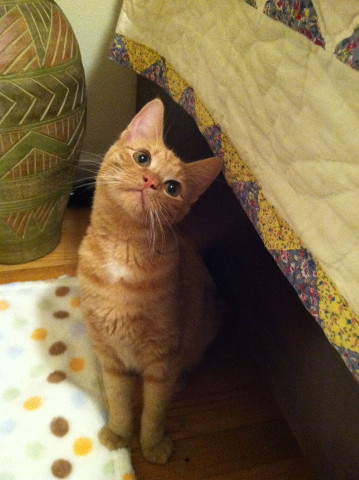
\includegraphics[width=0.58\textwidth]{images/cat}
\caption{A cat.}
\label{i:cat}
\end{figure}


As \cite{o2014cats} pointed out, there were many videos~\citep{o2014cats}.

%\chapter{Related Work}
\label{c:related}

\section{First}
\label{s:related1}

This is English line spacing test. You should see double spacing text.
This is English line spacing test. You should see double spacing text.
This is English line spacing test. You should see double spacing text.
This is English line spacing test. You should see double spacing text.
This is English line spacing test. You should see double spacing text.
This is English line spacing test. You should see double spacing text.
This is English line spacing test. You should see double spacing text.
This is English line spacing test. You should see double spacing text.
This is English line spacing test. You should see double spacing text.
This is English line spacing test. You should see double spacing text.
This is English line spacing test. You should see double spacing text.
This is English line spacing test. You should see double spacing text.
This is English line spacing test. You should see double spacing text.
This is English line spacing test. You should see double spacing text.
This is English line spacing test. You should see double spacing text.
This is English line spacing test. You should see double spacing text.
This is English line spacing test. You should see double spacing text.
This is English line spacing test. You should see double spacing text.
This is English line spacing test. You should see double spacing text.
This is English line spacing test. You should see double spacing text.
This is English line spacing test. You should see double spacing text.
This is English line spacing test. You should see double spacing text.
This is English line spacing test. You should see double spacing text.
This is English line spacing test. You should see double spacing text.

\section{Second}

This is English line spacing test. You should see double spacing text.
This is English line spacing test. You should see double spacing text.
This is English line spacing test. You should see double spacing text.
This is English line spacing test. You should see double spacing text.
This is English line spacing test. You should see double spacing text.
This is English line spacing test. You should see double spacing text.
This is English line spacing test. You should see double spacing text.
This is English line spacing test. You should see double spacing text.
This is English line spacing test. You should see double spacing text.
This is English line spacing test. You should see double spacing text.
This is English line spacing test. You should see double spacing text.
This is English line spacing test. You should see double spacing text.
This is English line spacing test. You should see double spacing text.
This is English line spacing test. You should see double spacing text.
This is English line spacing test. You should see double spacing text.
As discussed in Section~\ref{s:related1} and Chapter~\ref{c:related}.

%\input{photoshoot}
%\input{modeling}
%\input{application}
%\chapter{Conclusions}
\label{c:conclusion}


\appendix

\backmatter

\addcontentsline{toc}{chapter}{\bibname}
\bibliographystyle{abbrv}

% Your bibliography goes here
\bibliography{thesis}

\end{document}
